%%%%%%%%%%%%%%%%%%%%%%%%%%%%%%%%
\section{Materials and Methods}
%%%%%%%%%%%%%%%%%%%%%%%%%%%%%%%%
%
%-------------------------------
\subsection{Children}
%-------------------------------
%
Thirty two ($32$) children were selected using a large corpus of \textit{spontaneously spoken speech}, collected by the Computational Linguistics, Psycholinguistics and Sociolinguistics research center (CLiPS). The selection followed a two step procedure, similar to one outlined in \citet{Faes_et_al_2021}. First, a \textcolor{blue}{convenient sample} of hearing impaired children was selected based on the quality of their registered stimuli (utterances). And second, a \textcolor{blue}{matched sample} of normal hearing children was also selected.

For the first step, the \textcolor{blue}{convenient sample} of $16$ hearing impaired children with cochlear implant (HI/CI) were all native speakers of Belgian Dutch, living in Flanders, the Dutch speaking area of Belgium. They were all raised in monolingual Dutch with a limited support of signs, and all were screened as hearing impaired by the Universal Neonatal Hearing Screening (UNHS) using automated Auditory Brainstem Response hearing tests for newborns. After the identification of their hearing loss, the children were referred to a specialized audiological center for further audiological workup.

For the second step, $12$ normal hearing children (NH) are matched on gender, age, and regional background, to the groups selected in the previous step. The matching is done through a \textcolor{blue}{Manual or Propensity Score Matching (PSM)} procedure, \textcolor{red}{explain the appropriate procedure}.

Finally, the researcher considers important to highlight two relevant points from the children's selection process. First, while the matching procedure for the NH group uses the child's \textit{age} (at recording), the method cannot use the same variable for the other two groups. This is due to the fact that \textit{age} is merely used as a proxy, for the amount of time a child has been developing his(her) language. In that sense, more appropriate variables to use under the HI/CI and HI/HA groups would be e.g. the \textit{device length of use}, which approximates the "hearing age" of such children, or their \textit{vocabulary size}, which resembles their "lexical age" \citep{Faes_et_al_2021}. For this research, we consider the \textit{device length of use} as the simplest one to implement. Second, due to the nature of the sample selection procedure, we cannot ensure the HI/CI and HI/HA, nor the NH group, are representative of their respective populations. Therefore, inferences beyond this particular set of children must be taken with care.

\begin{comment}
	%%%%%%%%%%%%%%%%%%%%%%%%%%%%%%%%%%%%
	\textbf{for the experimenter:} Based on \citet{Faes_et_al_2021} we depict the procedure for the experimenter:
	%
	\begin{enumerate}
		\item 1. matching procedure 
		\item selection of suitable stimuli
		\item determine the number of stimuli per judge 
		\item 
	\end{enumerate}	
\end{comment}
%
%
%-------------------------------
\subsection{Stimuli} \label{ss:stimuli}
%-------------------------------
%
The stimuli consisted of the children's utterances (sentences of similar length) recovered from previously mentioned CLiPS corpus. More specifically, we use a portion of the corpus that consisted of $10$ utterances recordings, for each of the $32$ selected children. The stimuli were documented when the child was telling a story cued by the picture book "Frog, where are you" \citep{Mayer_1969} to a caregiver "who does not know the story". The quality of the stimuli was ensured by selecting utterances with no syntactically ill-formed or incomplete sentences, any background noise, cross-talk, long hesitations, revisions or non-words \citep{Boonen_et_al_2021}. 

As a result, the data set consisted in a total of $320$ utterances\footnote{under the Design of Experiments (DoE) literature, we would say we have $32$ experimental units with $10$ replicate runs each, making a total of $320$ experimental runs. As it is defined in \citet{Lawson_2015}, an experimental unit is the item under study upon which something is changed, while a replicate run is the experiment conducted with the same factor settings, but using different experimental units.} presented to the listeners in a random order, based on the adaptive pairing algorithm \citep{Pollitt_2012b} implemented in Comproved\footnote{evidence suggest that the number of comparisons and pairing algorithm impacts the reliability, validity and efficiency of the procedure \citep{Bramley_2015, Bramley_et_al_2018, Lesterhuis_2018, Verhavert_et_al_2019}. However, this is not investigated in the current research.}.

Similar designs were used by \citet{Boonen_et_al_2020} and \citet{Faes_et_al_2021}. However, in the former case the number of samples were low, while in the latter, the design was unbalanced and not conducive to appropriate inferences from the pairwise comparisons.



%-------------------------------
\subsection{Experimental setup}
%-------------------------------
%
On both procedures, the experimental settings for the \textbf{judgment task} followed the next steps \citep{Boonen_et_al_2020, Boonen_et_al_2021}:
%
\begin{enumerate} \itemsep1pt
	\item the listener take a seat in front of a computer screen, located at his(her) home, workplace, or the experimental laboratory.
	%
	\item the listener open Comproved\footnote{software developed by the University of Antwerp designed to perform comparative judgments: \url{https://comproved.com/en/a}.} and select the rating task.
	%
	\item the listener read two set of instructions presented on the computer screen about:
	\begin{enumerate}
		\item how to perform the task, and
		\item the aspects not to consider for the task.
	\end{enumerate}
	%
	\item the listener hear the stimuli through high quality headphones, set at a comfortable volume.
	%
	\item the listener rate which stimulus sounded more intelligible by selecting the appropriate button, for CJ-D and CJ-O tasks, or a score from a slider on the computer screen, for the HJ task.
	%
	\item \textcolor{blue}{the listener provide a decision statement on why the selected stimulus sounded more intelligible.}
\end{enumerate}
%
\begin{figure}[h]
	\centering
	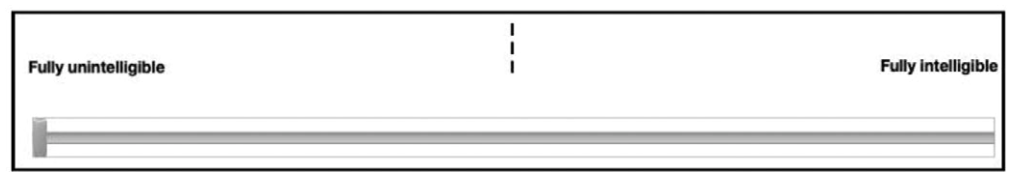
\includegraphics[width=0.8\linewidth]{slider.png}
	%
	\caption[Slider for the HJ task.]%
	{Slider for the HJ task. Extracted from \citet{Boonen_et_al_2021}.}
	\label{fig:slider}
\end{figure}
%
Observational evidence indicate the HJ procedure might suffer from anchoring effects\footnote{a bias in decision that occurs when people anchor their decisions around a reference point, and adjust their choices relative to it \cite{Baddeley_2017, Kahneman_2013}.} or issues with the default option of the slider. About the former, the anchoring seem to happen when listeners consider the previous assessment as a reference point for the next, effectively turning the task into a comparative rating, similar to CJ. About the latter, as the default setting for the slider is located on the far left for each new assessment (as seen in Figure \ref{fig:slider}), it is likely that such setting might impact the rating procedure\footnote{compelling evidence on how default settings impact several decision process can be found in \citet{Kahneman_2013} and \citet{Johnson_et_al_2003}.}. Considering the previous, in order to minimize both issues, care is taken to randomize the display of stimuli within each listener. However, the researcher recognizes that a better approach to face the second problem would be to randomize the default setting of the slider, but this will not be applied nor investigated on the current research. 

\textcolor{red}{talk about decision statements or thinking-at-loud tasks.}

Finally, for the \textbf{transcription task}, the followed steps were similar to the previous task. Although, at the fourth step, the listeners did not rated the stimulus but rather wrote their orthographic transcriptions, in a free text field in the Comproved environment.


On the other hand, for the transcription task, $100$ transcribers participated in the experiment. The participants and stimuli were divided into five groups, where each group of $20$ students ($100/5$) transcribed $64$ stimuli on their series ($320/5$), resulting in $20$ transcriptions per utterance ($64 \times 100 / 320$). In total we registered $6400$ transcriptions\footnoteref{foot:doe}}.
